\documentclass[11pt]{article}
\usepackage[margin=1in,footskip=0.25in]{geometry}
\usepackage{setspace}
\usepackage{titlesec}
\usepackage{pgf-pie} 
\usepackage{authblk}
%\usepackage{hyperref}
\usepackage{listings}
\usepackage{graphicx}
\usepackage{subcaption}
\usepackage{adjustbox}
\usepackage{booktabs}
\usepackage[normalem]{ulem}
\graphicspath{ {./images/} }










\titleformat{\chapter}
  {\Large\bfseries} % format
  {}                % label
  {0pt}             % sep
  {\huge}           % before-code
\onehalfspacing
%\doublespacing
\begin{document}
\begin{titlepage}
% 
\includegraphics[scale = 1]{images/iitjammu.jpg}
\font\myfont=cmr12 at 40pt
\author{\normalsize {Rajat Mittal}} 
\affil{\normalsize{M.Tech. Computer Technology}}
\affil{\normalsize{Student ID - 2020PCT0066}}
\affil{\normalsize {Email: 2020PCT0066@iitjammu.ac.in}}



\title{\myfont A Web Crawler}

\maketitle
\centering{
\includegraphics[scale = 1]{images/iitjammu.jpg}}
\end{titlepage}

\pagebreak
% \addtocounter{page}{1}
\centerline{\uline{\Large{\textbf{A Text - Crawler}}}}
\subsection*{Crawled Website:- https://books.toscrape.com/}

\hspace{1in}In the Text-Crawler, I crawled a bookstore website. This website has around 1000 books in 50 pages. I crawled all of them using Python libraries.
\\

\hspace{Libraries used: \textbf{BeautifulSoup, requests, csv}} \\
\rule{\textwidth}{0.4pt}
\textbf{Text Crawler} Python Code for text-crawling\\
\rule{\textwidth}{0.4pt}
\begin{lstlisting}
# import necessary libraries
import requests
from bs4 import BeautifulSoup
import csv


# adding given urls
url = "https://books.toscrape.com/"

# get the html content
r = requests.get (url)

html_content = r.content

# making the soup - parsing the HTML
soup = BeautifulSoup (html_content, 'html.parser')

data = []

catalogue = soup.find_all ("ol", {"class":"row"})

for item in catalogue [0].find_all ("li", {"class":"col-xs-6 col-sm-4 col-md-3 col-lg-3"}):
  mdata = {}
  mdata ['title'] = item.h3.a.get ("title")
  mdata ['rating'] = item.p.get ("class") [1]
  mdata ['price'] = item.find ("p", {"class":"price_color"}).text
  mdata ['stock'] = item.find ("p", {"class":"instock availability"}).text [15:17]
  data.append (mdata)

#Save into CSV file

file_csv = 'book-store.csv'

with open (file_csv, 'w', newline='') as f:
    w = csv.DictWriter (f, ['title', 'rating', 'price', 'stock'])
    w.writeheader ()
    for mdata in data:
        w.writerow (mdata)



\end{lstlisting}
\rule{\textwidth}{0.4pt}

\subsection*{Sample Output Photo}
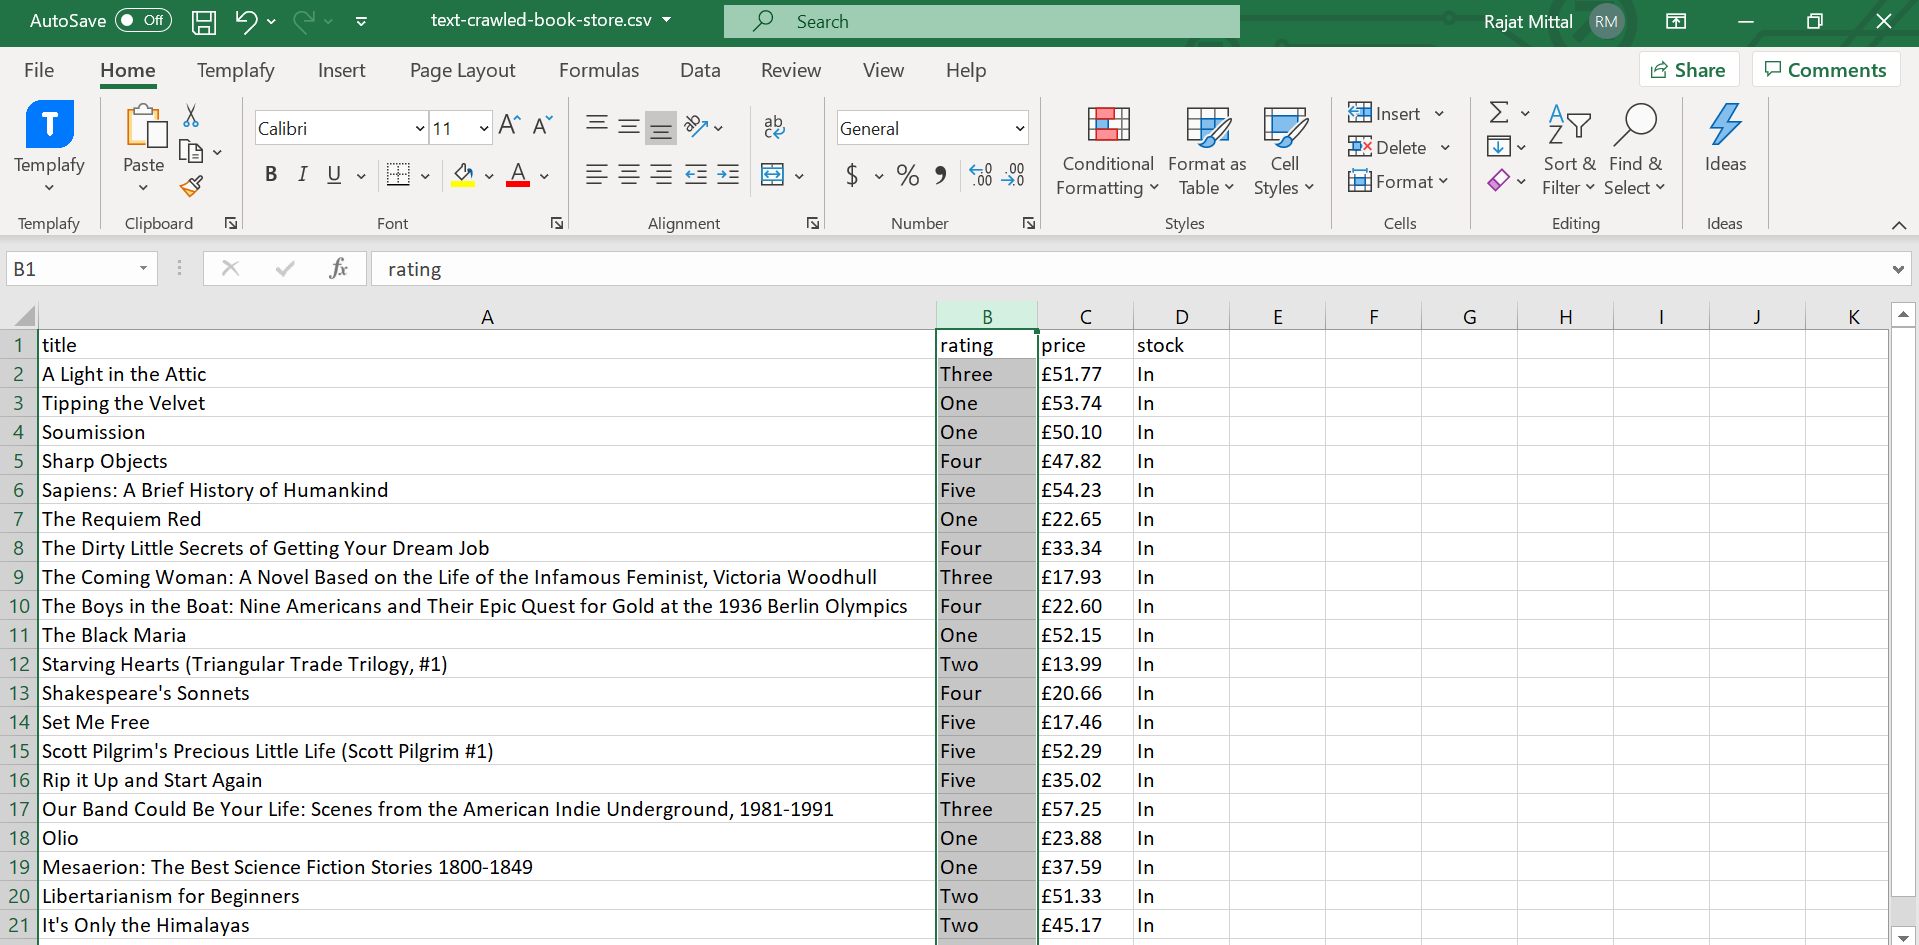
\includegraphics[scale=0.5]{images/Text-crawled.PNG}

\pagebreak
\centerline{\uline{\Large{\textbf{An Image - Crawler}}}}
\subsection*{Crawled Website:- https://books.toscrape.com/}

\hspace{1in}In the Image-Crawler, I crawled a bookstore website. This website has around 1000 books in 50 pages. Also it has image for every book. So, I crawled all images of books using Python libraries.
\\

\hspace{Libraries used: \textbf{BeautifulSoup, requests, os}} \\
\rule{\textwidth}{0.4pt}
\textbf{Image Crawler} Python Code for images-crawling\\
\rule{\textwidth}{0.4pt}
\begin{lstlisting}
import requests
from bs4 import BeautifulSoup
import os

data = []
images = []
image_url = "https://books.toscrape.com"
# add your url
for i in range(1,51):
    url = "https://books.toscrape.com/catalogue/page-" + str(i) + ".html"
    #print(url)
    r = requests.get (url)
    html_content = r.content
    soup = BeautifulSoup (html_content, 'html.parser')
    catalogue = soup.find_all("img")
    
    
    for image in catalogue:
      images.append(image['src'])

for i in range(len(images)):
  temp = images[i][2:]
  images[i] = image_url+temp
  #print(image)


os.mkdir('Rajat_photos')
i = 1

for index, img_link in enumerate(images):
    if i <= len(images):
        img_data = requests.get(img_link).content
        with open("my_pics/"+str(index+1)+'.jpg', 'wb+') as f:
            f.write(img_data)
        i += 1
    else:
        f.close()
        break

\end{lstlisting}
\rule{\textwidth}{0.4pt}

\subsection*{Sample Output Photo}
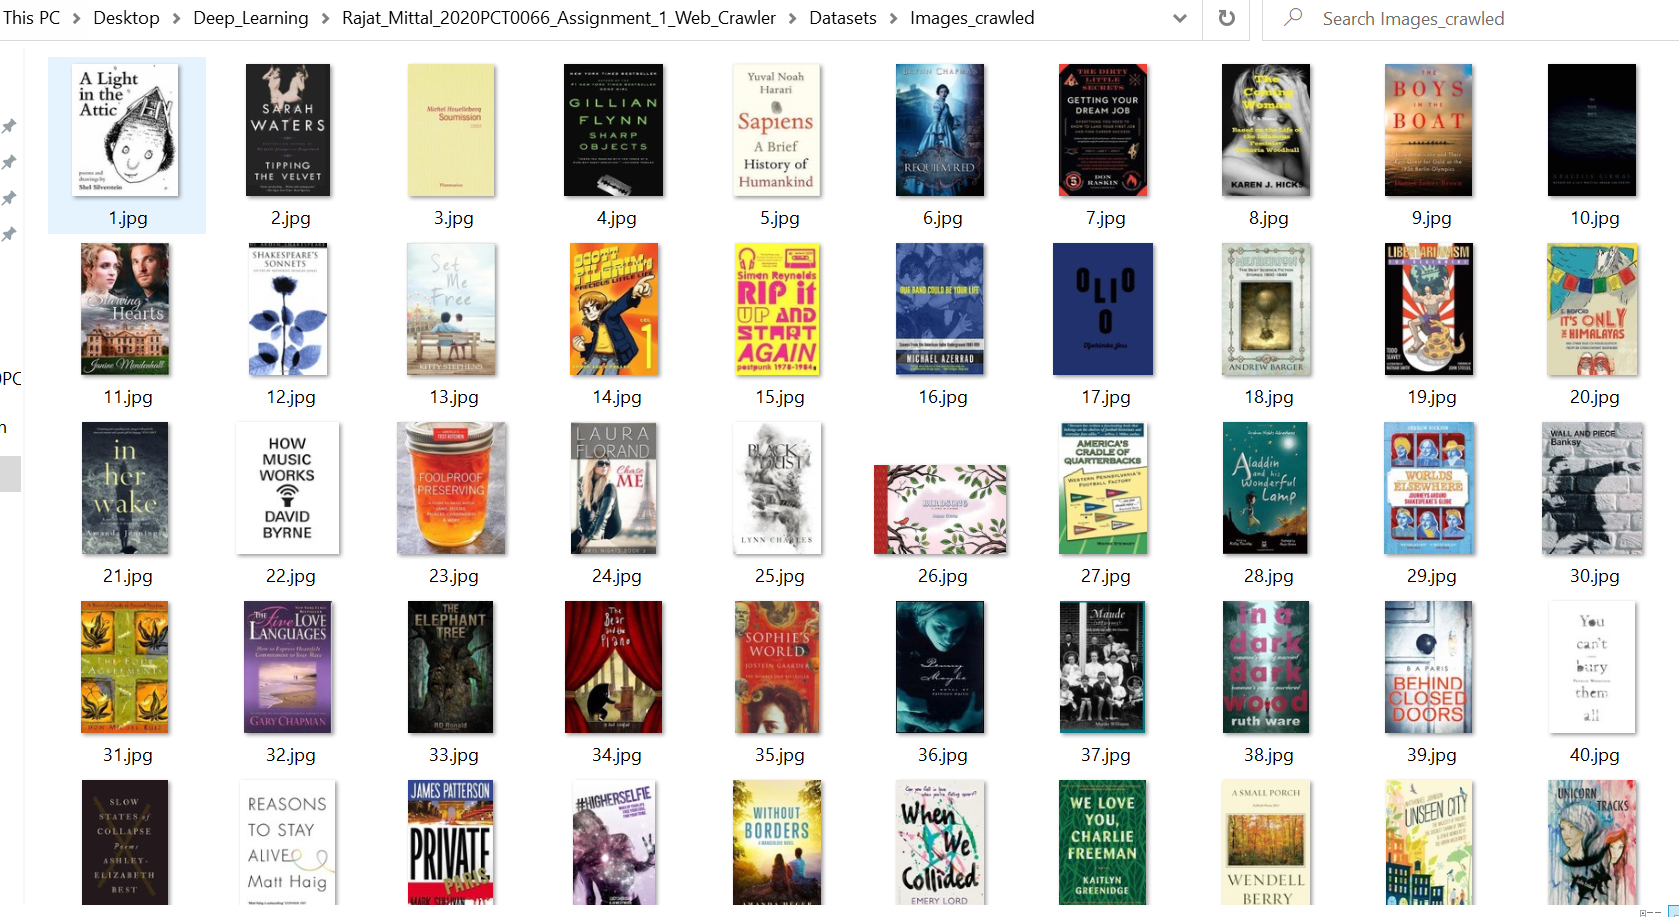
\includegraphics[scale=0.5]{images/Images-crawled.PNG}
\pagebreak

\centerline{\uline{\Large{\textbf{A Video - Crawler}}}}
\subsection*{Crawled Website:- https://sample-videos.com/}

\hspace{1in}In the Video-Crawler, I crawled a sample video website.In a one video page of that webiste, it has around 80+ videos. I crawled all of them using Python libraries. It has .mp4, .3gp and .flv videos.

\\

\hspace{Libraries used: \textbf{BeautifulSoup, requests}} \\
\rule{\textwidth}{0.4pt}
\textbf{Videos Crawler} Python Code for videos-crawling\\
\rule{\textwidth}{0.4pt}
\begin{lstlisting}
import requests
from bs4 import BeautifulSoup

links = []
videos = []

videos_url = "https://sample-videos.com/"

url = "https://sample-videos.com/index.php#sample-mp4-video"

r = requests.get (url)
html_content = r.content
soup = BeautifulSoup (html_content, 'html.parser')

for a in soup.find_all('a', href=True):
    videos.append(a['href'])

videos = videos[26:len(videos)-1]


for i in range(len(videos)):
  links.append(videos_url + videos[i])

def download_video_series(video_links):
	for link in video_links:
		file_name = link.split('/')[-1]
		r = requests.get(link, stream = True)
		with open(file_name, 'wb') as f:
			for chunk in r.iter_content(chunk_size = 1024*1024):
				if chunk:
					f.write(chunk)
	return
#temp = links[0:2]

download_video_series(links)

\end{lstlisting}
\rule{\textwidth}{0.4pt}

\subsection*{Sample Output Photo}
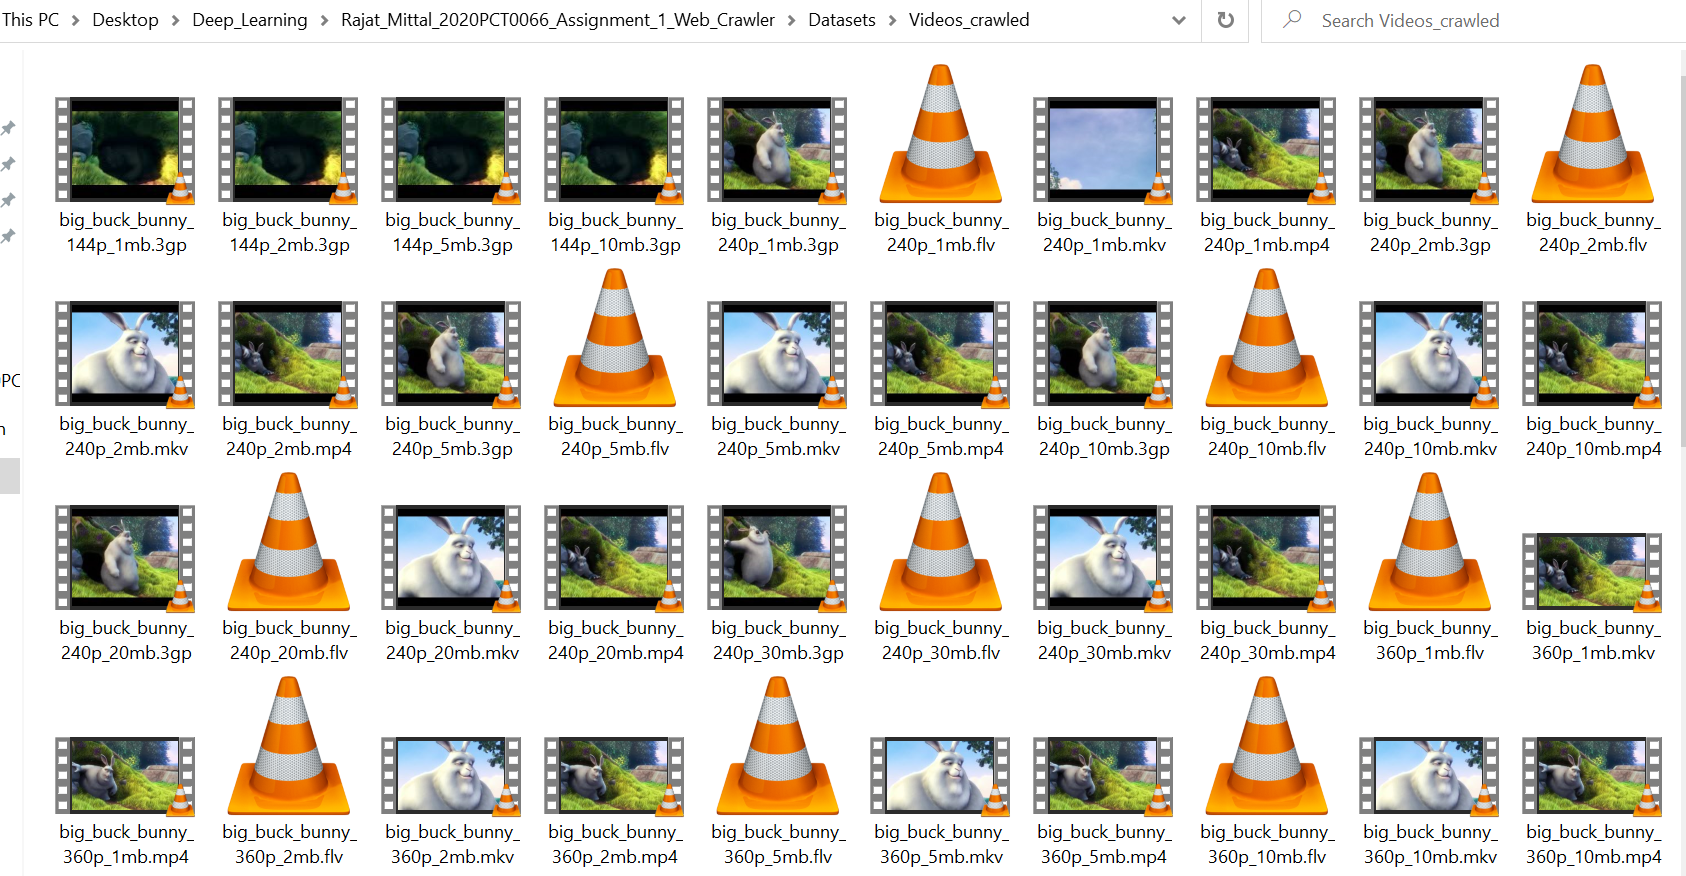
\includegraphics[scale=0.5]{images/Videos-crawled.PNG}

\pagebreak


\font\myfont=cmr12 at 40pt
\centering{\myfont Thank You!}


\end{document}